%%%%%%%%%%%%%%%%%%%%%%%%%%%%%%%%%%%%%%%%%
% Journal Article
% LaTeX Template
% Version 1.3 (9/9/13)
%
% This template has been downloaded from:
% http://www.LaTeXTemplates.com
%
% Original author:
% Frits Wenneker (http://www.howtotex.com)
%
% License:
% CC BY-NC-SA 3.0 (http://creativecommons.org/licenses/by-nc-sa/3.0/)
%
%%%%%%%%%%%%%%%%%%%%%%%%%%%%%%%%%%%%%%%%%
%----------------------------------------------------------------------------------------
%       PACKAGES AND OTHER DOCUMENT CONFIGURATIONS
%----------------------------------------------------------------------------------------
\documentclass[paper=letter, fontsize=12pt]{article}
\usepackage[ruled,vlined]{algorithm2e}
\usepackage[english]{babel} % English language/hyphenation
\usepackage{amsmath,amsfonts,amsthm} % Math packages
\usepackage[utf8]{inputenc}
\usepackage{float}
\usepackage{lipsum} % Package to generate dummy text throughout this template
\usepackage{blindtext}
\usepackage{graphicx} 
\usepackage{caption}
\usepackage[table]{xcolor}
\usepackage{subcaption}
\usepackage[sc]{mathpazo} % Use the Palatino font
\usepackage[T1]{fontenc} % Use 8-bit encoding that has 256 glyphs
\linespread{1.05} % Line spacing - Palatino needs more space between lines
\usepackage{microtype} % Slightly tweak font spacing for aesthetics
\usepackage[hmarginratio=1:1,top=32mm,columnsep=20pt]{geometry} % Document margins
\usepackage{multicol} % Used for the two-column layout of the document
%\usepackage[hang, small,labelfont=bf,up,textfont=it,up]{caption} % Custom captions under/above floats in tables or figures
\usepackage{booktabs} % Horizontal rules in tables
\usepackage{float} % Required for tables and figures in the multi-column environment - they need to be placed in specific locations with the [H] (e.g. \begin{table}[H])
\usepackage{hyperref} % For hyperlinks in the PDF
\usepackage{lettrine} % The lettrine is the first enlarged letter at the beginning of the text
\usepackage{paralist} % Used for the compactitem environment which makes bullet points with less space between them
\usepackage{abstract} % Allows abstract customization
\renewcommand{\abstractnamefont}{\normalfont\bfseries} % Set the "Abstract" text to bold
\renewcommand{\abstracttextfont}{\normalfont\small\itshape} % Set the abstract itself to small italic text
\usepackage{titlesec} % Allows customization of titles

%\renewcommand\thesection{\Roman{section}} % Roman numerals for the sections
%\renewcommand\thesubsection{\Roman{subsection}} % Roman numerals for subsections

\titleformat{\section}[block]{\large\scshape\centering}{\thesection.}{1em}{} % Change the look of the section titles
\titleformat{\subsection}[block]{\large}{\thesubsection.}{1em}{} % Change the look of the section titles
\newcommand{\horrule}[1]{\rule{\linewidth}{#1}} % Create horizontal rule command with 1 argument of height
\usepackage{fancyhdr} % Headers and footers
\pagestyle{fancy} % All pages have headers and footers
\fancyhead{} % Blank out the default header
\fancyfoot{} % Blank out the default footer

\fancyhead[C]{Journey Risk Management : IOCL Dimapur Depot} % Custom header text

\fancyfoot[RO,LE]{\thepage} % Custom footer text
%----------------------------------------------------------------------------------------
%       TITLE SECTION
%----------------------------------------------------------------------------------------
\title{\vspace{-15mm}\fontsize{24pt}{10pt}\selectfont\textbf{Journey Risk Management Study : IOCL Dimapur Depot}} % Article title
\author{
\large
{{\textbf{Committee Members} }}\\
{{Mr. S M Rajkumar$^*$, SOO(Safety) \& Mr. H Hazarika$^{**}$, AM(Ops.-IM)}}\\
{{\textbf{Reviewer:} Mr. Mudang Tacho$^{***}$, CDM}}\\
%\thanks{A thank you or further information}\\ % Your name
\normalsize \href{mailto:mohanrs@indianoil.in}{$^*$mohanrs@indianoil.in}, \href{mailto:hazarikah@indianoil.in}{$^{**}$hazarikah@indianoil.in}, \href{mailto:mtacho@indianoil.in}{$^{***}$mtacho@indianoil.in}\\[2mm] % Your email address
}
\date{}

%----------------------------------------------------------------------------------------
\begin{document}
\maketitle % Insert title
\thispagestyle{fancy} % All pages have headers and footers


\tableofcontents

\section{Introduction}

The most significant contributor of traumatic injury at work is the use of vehicle in road traffic \cite{aus}. There are 1635 road accidents during transportation reported by Indian  oil and gas companies in the last five years \cite{accident}. As per \cite{retzer1}, motor vehicle fatality rate in oil and gas industry is many folds more than all other industry. The major measures to prevent motor vehicle job-related fatalities are \cite{retzer1}:

\begin{itemize}
    \item Decreasing the total amount of travel.
    \item Seeking alternate means of transport if possible.
    \item Reducing the risks associated with road transport.
    \item Reducing crash severity to reduce injury severity.
\end{itemize}

IOCL Dimapur Depot deals with POL products which come under essential commodities. Therefore, reducing the amount of travel for POL tank trucks (TTs) is not an option as POL products need to reach every nook and corner of the state of Nagaland. There is currently no other transport infrastructure available in Nagaland to transport POL products. Prevention of crash severity may reduce injury severity, but there may be other disasters arising due to crash of POL transport vehicles (e.g. fire, soil / water pollution etc.). Therefore, the only viable measure for reducing POL transport-related motor vehicle fatalities is to reduce risks associated with road journey. Journey Risk Management is a promising preventive measure to reduce road travel related risks \cite{retzer1}.



\subsection{Risk \& Risk Management}
Risk in supply-chain refers to unimaginable events that might happen in future causing disturbance to the smooth supply of materials \cite{waters}. The major feature of risk is that it is somewhat quantifiable which comes out to be handy in eliminating it \cite{waters}. The concept of risk can therefore be linked to probability of an unforeseen and undesired event. There can be three ways of finding probability of an event \cite{waters}:

\begin{enumerate}
    \item \textbf{Calculation}: Prior knowledge of an event or situation is used to compute probability. 
    \begin{equation}
        Probability = \frac{Number\, of\, ways\, of\, occurrence\, of\, the\, event}{Total\, possible\, outcomes}
    \end{equation}
    \item \textbf{Observation}: Historical information on frequency of occurrence of an event can be used to calculate observation based or empirical probability.
    \begin{equation}
        Probability = \frac{Number\, of\, times\, of\, occurrence\, of\, the\, event}{Total\, number\, of \, observations}
    \end{equation}
    \item \textbf{Subjective estimation}: People's opinion and judgements can be used to determine likelihood of an event. But, one should always carefully scrutinize before accepting subjective estimates.
\end{enumerate}

Risk management revolves around three major activities: identification of risks, analysis of their consequences,developing germane measures to control risks, and review of control measures \cite{waters} \cite{aus}. A superior approach to manage risk is proactive analysis of likely events beforehand and planning steps to alleviate their effects \cite{waters}


 \begin{figure}[htpb]
    \centering
    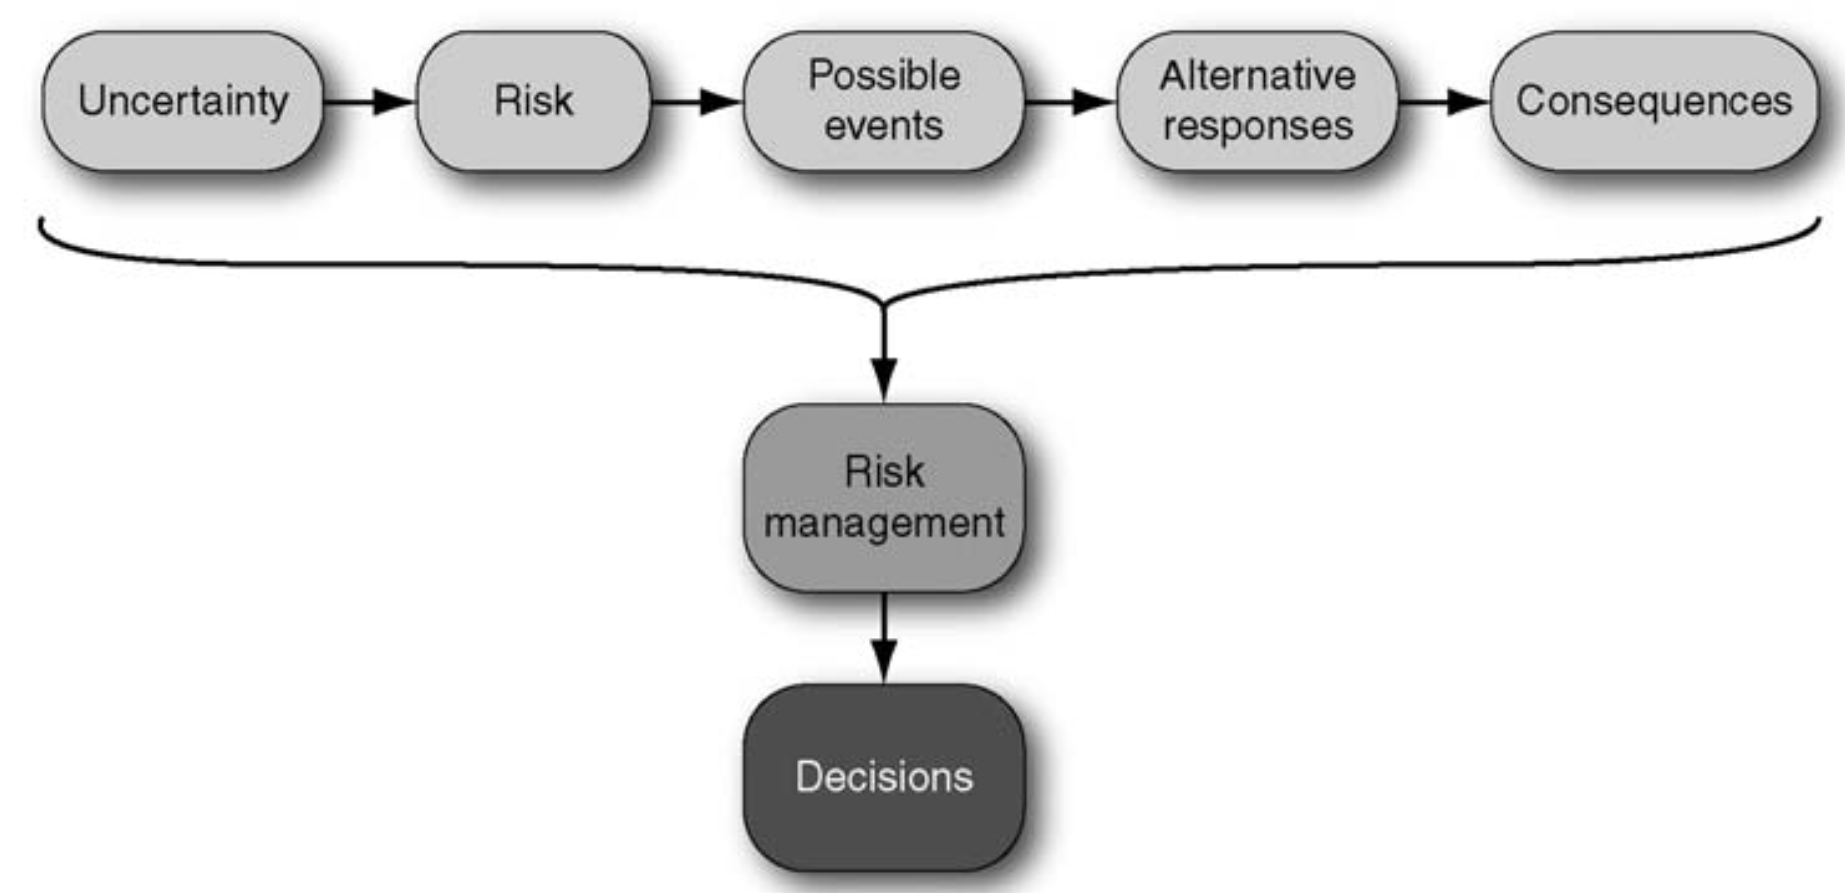
\includegraphics[scale = 0.4]{risk1}
    \caption{The basic risk management process}
    \label{risk_management}
\end{figure}



\subsection{Basic Idea of Journey Risk Management}
Journey Risk Management points to organized and planned process for minimizing transportation-related risks within a organization's operations \cite{retzer1}. As part of JRM study, a general risk assessment is conducted which covers assessment of the driver, the vehicle type, route to be travelled, weather, time of the day, and distance \cite{retzer2}.
The assessment of the driver generally comprises minimum qualifications, hours of sleep, and hours of service. Vehicle assessment includes corroboration that the vehicle is germane to the journey and a confirmation of completed pre-trip inspection \cite{retzer2}. Route risk assessments are completed on main roads and are evaluated prior to each trip \cite{retzer2}. Being declared as essential commodities in India, petroleum products (eg. MS, SKO, HSD) need to reach every nook and corner of the country regardless of the geography, difficulty level of the driving terrain, and adverse weather conditions.

\subsection{Need of Journey Risk Management}

POL installations are controlled and supervised environments in terms of safety and health with prolific safety and health related measures, policies, and procedures. But, once POL TTs leave the installation premises, the environment becomes unsupervised. Also, the driving environment becomes uncontrolled with lots of public third party drivers. Moreover, the operating conditions may also change constantly. Petroleum products like MS, HSD, SKO etc. being essential commodities, some level pressure is always there on the POL TT drivers to reach the destination on  time. This may result in unsafe practices by TT drivers and also may make it difficult to manage the changing environment and operating conditions \cite{retzer1}. In order to address these issues, Journey Risk Management needs to be adopted by supervisors of POL supply chain managers.



\section{Development of Journey Risk Management Plan (JRMP)}

In this section, step by step procedure to develop JRMP in relevance to POL trasnportation will be discussed with the help of \cite{retzer1}, \cite{waters}, \& \cite{pune}.

\subsection{Development of Road Safety Framework}
While developing a JRMP, first thing is to have a comprehensive road transport safety policy. At Indian Oil, there exists a thorough road transport safety policy which encapsulates motor vehicle act and hazardous good transport guidelines.

\subsection{Development of Risk Register}

A Risk register needs to be developed to spot overall driving vulnerability. For each driving activity, potential the hazards or operating conditions capable of causing motor vehicle incident is to be written down. In doing so, previous company lesson learnt circulars and input from TT drivers to be utilized. Finally, we have to jot down the risks or consequences that may occur out of each hazard. A sample risk register has been shown in figure \ref{risk_register}.

 \begin{figure}[htpb]
    \centering
    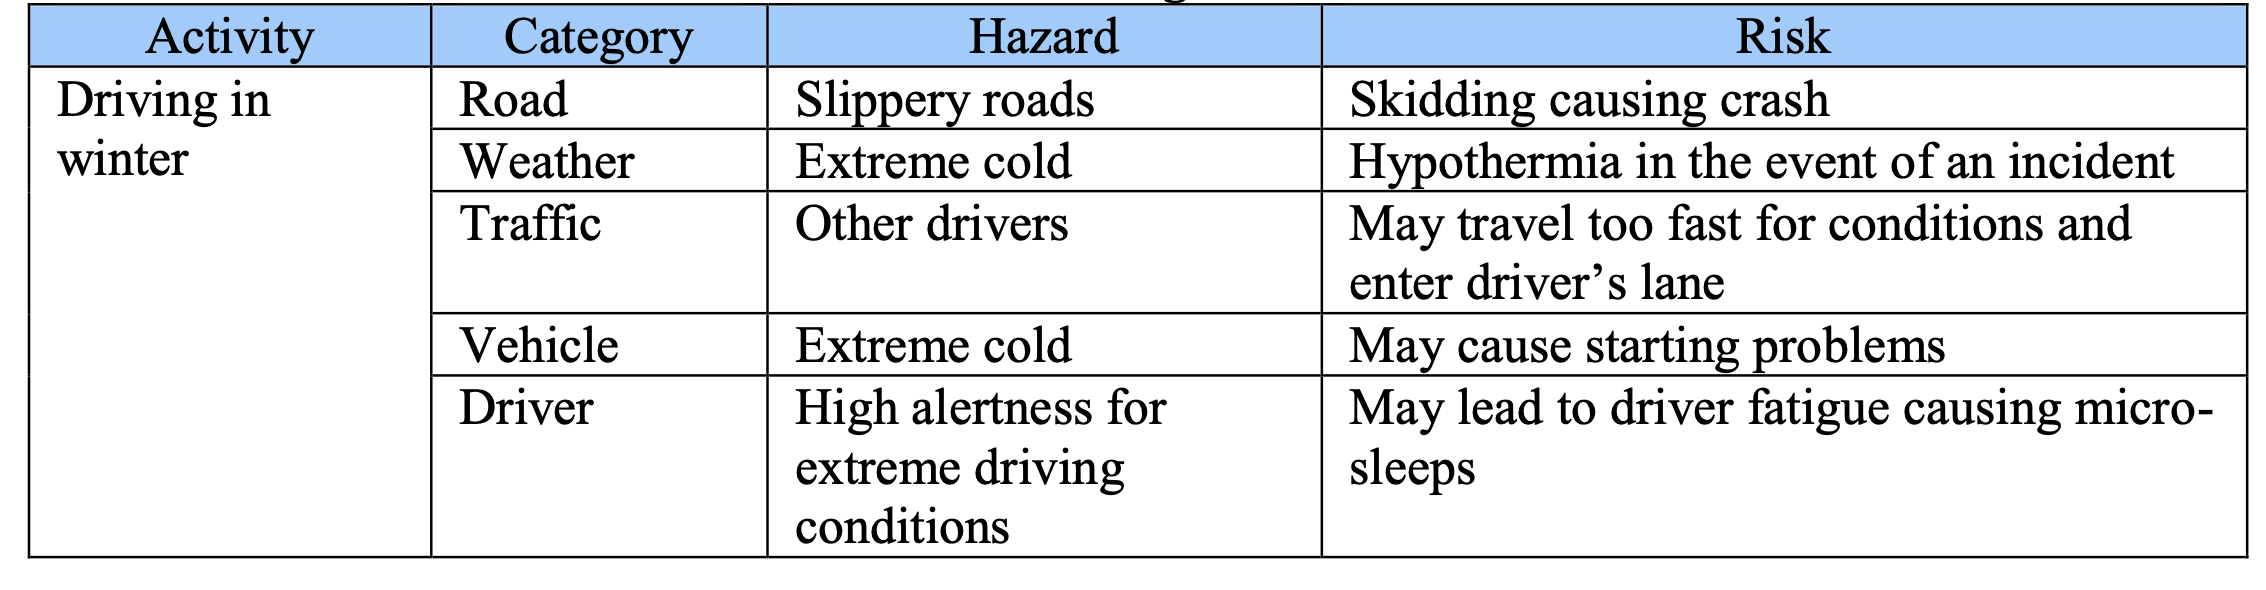
\includegraphics[scale = 0.4]{riskreg}
    \caption{A Sample Risk Register \cite{retzer1}}
    \label{risk_register}
\end{figure}


\subsection{Discovering Control Measures for Risks \& Risk Control Matrix}

We have to identify the control measure(s) to prevent or mitigate the risks listed in the risk register. Writing down this measures against each risk will give us the Risk Control Matrix. The JRMP planner should try to include all the control measures to best manage the risks encountered in road transportation. Those controls need to be pragmatic and consistent.
The risks can be rated with respect to the vulnerability of consequences (e.g. high, medium, low).

\subsection{Route Analysis}

Route data is collected to analyze the possible risk factors for driving difficulty for a particular trip. It will help to eradicate accidents and other emergencies in a journey. Risk rating to be given for every section of the trip along with possible control measures based on risk control matrix. A sample route analysis for one section has been shown below:\\




\setlength{\arrayrulewidth}{1mm}
\setlength{\tabcolsep}{18pt}
\renewcommand{\arraystretch}{2.5}

\newcolumntype{s}{>{\columncolor[HTML]{AAACED}} p{3cm}}

\arrayrulecolor[HTML]{DB5800}

\begin{tabular}{ |p{0.5cm}|p{2.5cm}|p{2cm}|p{3cm}|p{1cm}|  }
\hline
\rowcolor{lightgray} \multicolumn{5}{|c|}{Route Analysis} \\
\hline
Section& Route Data &Risk Factors & Control Measures& Risk Rating \\
\hline
1 & Dimapur Depot Exit Gate & T-juction with 2 way traffic& Use convex mirrors installed to monitor traffic \& use indicators of vehicle& \cellcolor[HTML]{FF0000} \textbf{High}\\
\hline
\end{tabular}

\subsection{En-route Considerations}

During the journey, drivers should monitor risks continuously and act as per the control measures. It is advisable for drivers to plan their rest stops, stoppage for meals, and to plan for avoiding distractions while driving. JRM plan may include possible rest spots, restaurants, hospitals, repair shops, and emergency contact numbers for the convenience of the driver.


\subsection{Post-trip Considerations}

Drivers should plan the return journey after competition of the trip. The plan starts with post trip vehicle inspection to ensure that the vehicle is fit for the next trip. Any changing risk factor / hazard during the journey and/or near miss to be reported to the journey managers (in our case POL depot/terminal's concerned officer) for improvement in the JRM plan.

\subsection{Creation of the JRM Plan}

The JRM plan is one single document including the road safety policy, risk register, risk controls, route analysis, en-route considerations, and post-trip considerations.

\section{JRM Plan for Route 1}

In this section JRM plan for for route 1 of 28 km distance from IOCL Dimapur Depot (25.890355, 93.723578) to Medziphema Auto Centre (25.757663, 93.847789) will be discussed.
A total of 12 number of IOCL retail outlets are covered in this route.
 \begin{figure}[htpb]
    \centering
    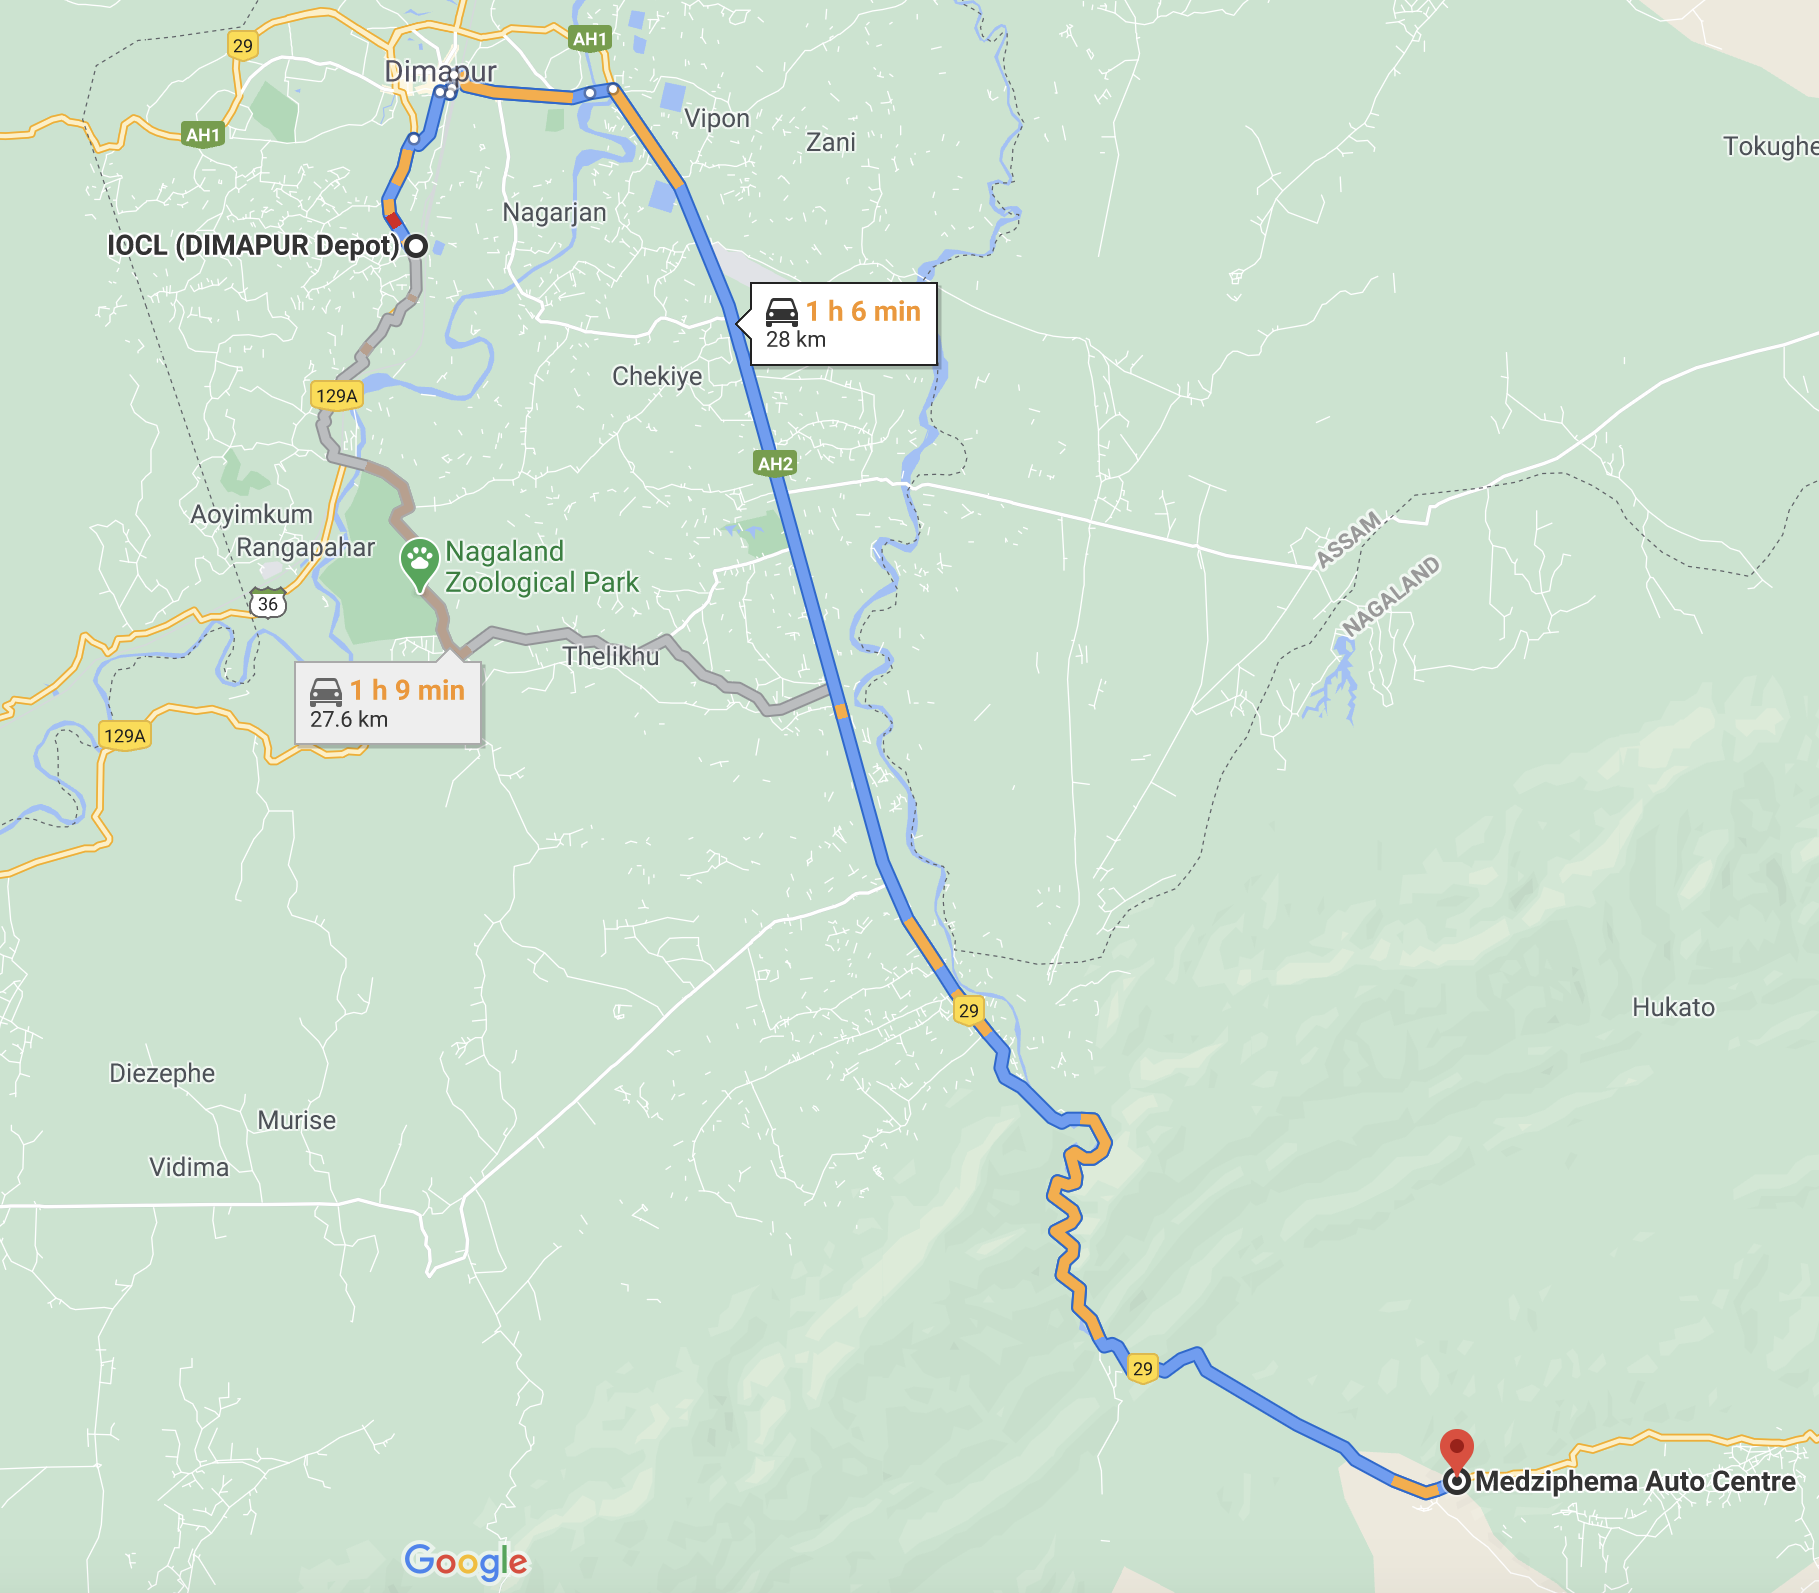
\includegraphics[scale = 0.4]{route1}
    \caption{Route 1 for JRM Plan}
    \label{route1}
\end{figure}

\subsection{Road Safety Framework for Route 1}

Indian Oil's tank truck movement framework is guided by Motor Vehicle Act and Industry Transport Discipline Guidelines (ITDG). Each tank truck need to comply with the following guidelines:

\begin{itemize}
    \item There should be one driver and one cleaner / helper for each tank truck.
    \item The driver need to possess a valid driving license for heavy vehicles (Transport category).
    \item The driver must undergo training on safe transportation of hazardous goods once in a year and their DL need to be endorsed by RTO for the training.
    \item Both the driver and helper must be provided with training as per OISD Std. 154 guidelines.
    \item Both the driver and helper should be in sound health condition. Therefore, periodic health and eye check up record to be kept.
    \item The maximum allowable speed for TT on load is 50 KMPH and the same for empty TT is 60 KMPH.
    \item The TT must follow the route approved by IOCL.
    \item The mandatory night rest / halt timing is from 22:00 Hrs to 06:00 Hrs. Therefore, the TT driver should refrain from driving during night post 22:00 Hrs.
    \item Contain one TREM (Transport Emergency) card.
    \item There should not be any deviation from the approved route for a considerably longer duration during a trip, unless there is any emergency or approval from competent authority.
    \item Vehicle Tracking System's VMU in working condition.
    \item There should be at least one 9/10 Kg DCP fire extinguisher and one 1/2 kg CO2 type fire extinguisher in  each TT.
    \item There should be one First aid box.
    \item Fire screen between cabin and tank.
    \item 300A battery cut off switch.
    \item Battery terminals must be covered.
    \item HAZCHEM signs must be clearly visible.
    \item The TT crews must comply with all other general traffic rules.
\end{itemize}


\subsection{Risk Control Matrix for Route 1}

The risk register was developed by augmenting all the possible risk factors for route 1. The risk control matrix was then developed taking into account of the risk factors included in the risk register. The risks considered are particularly relevant to route 1. For other routes, new risk factors may come and need to the incorporated accordingly. The risk control matrix for route 1 is shown as Figure \ref{rcm}.

\begin{figure}[htpb]
    \centering
    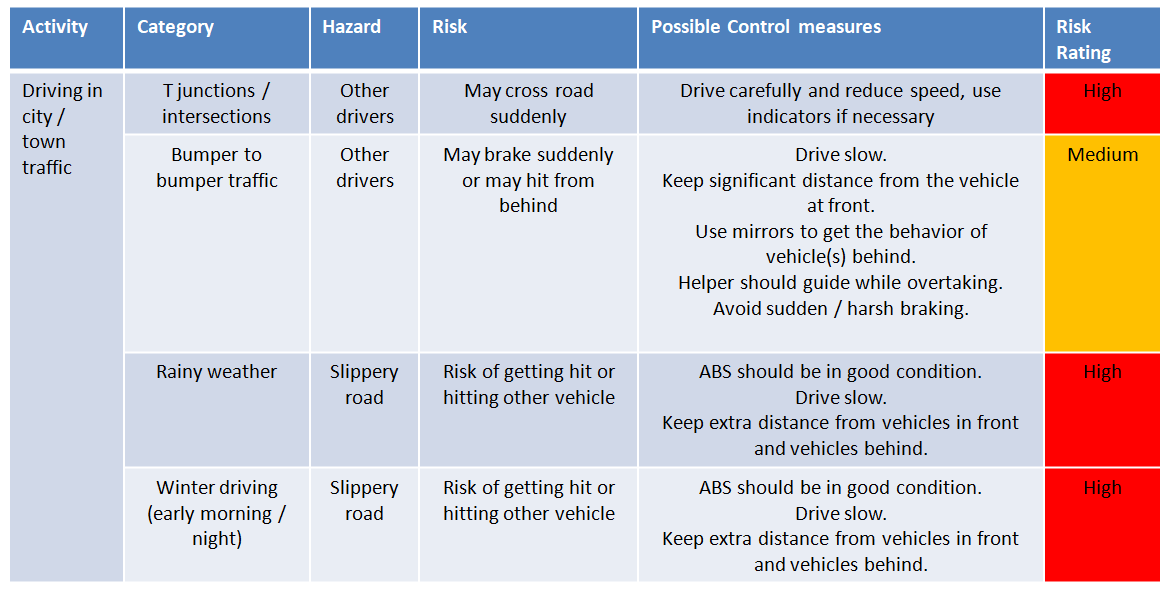
\includegraphics[scale = 0.412]{jrm1}
 
\end{figure}

\begin{figure}[htpb]
    \centering
    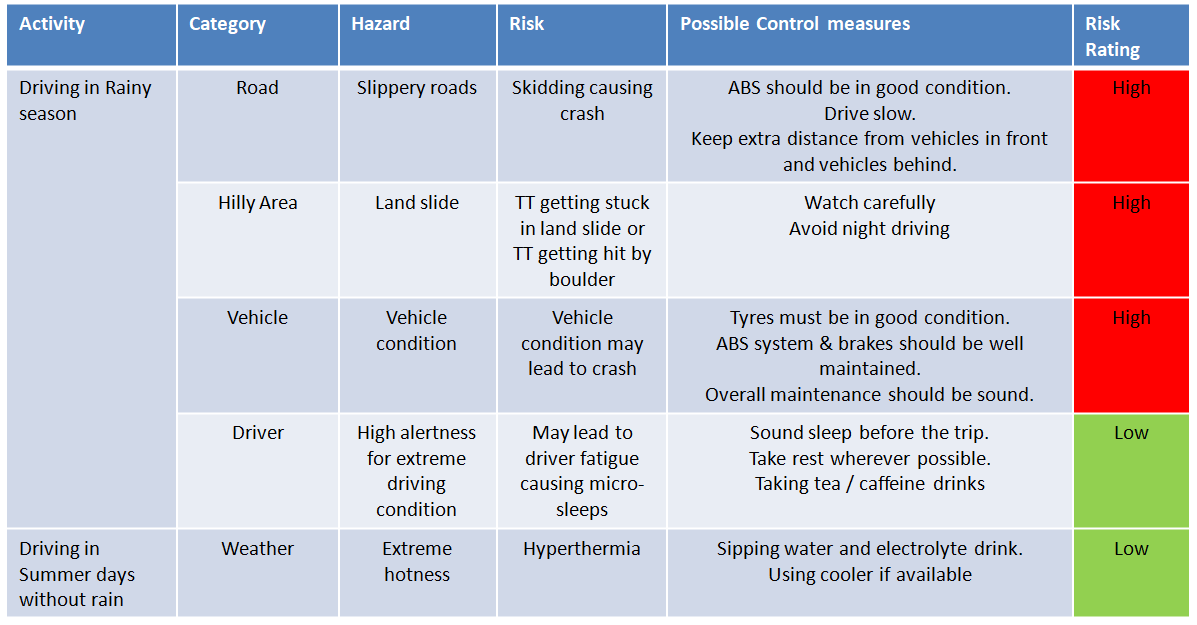
\includegraphics[scale = 0.4]{jrm2}
  
\end{figure}

\begin{figure}[htpb]
    \centering
    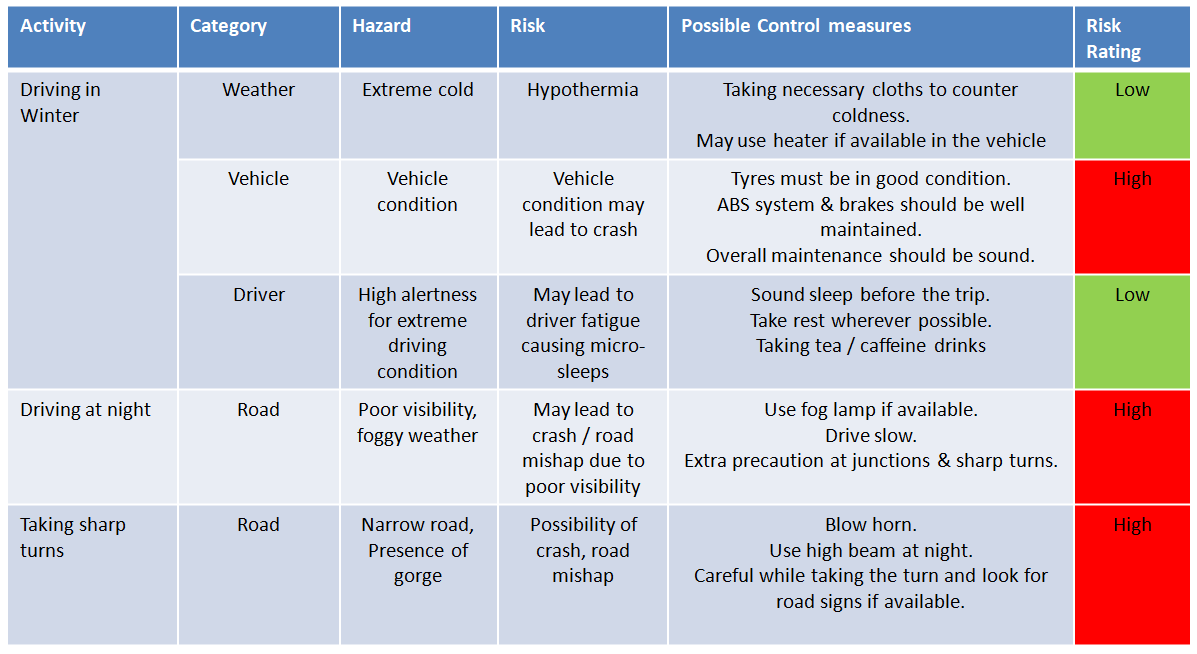
\includegraphics[scale = 0.4]{jrm3}
    \caption{Risk Control Matrix for Route 1}
    \label{rcm}
\end{figure}


\subsection{Analysis of Route 1}

\begin{tabular}{ |p{0.5cm}|p{2.5cm}|p{2cm}|p{3cm}|p{1cm}|  }
\hline
\rowcolor{lightgray} \multicolumn{5}{|c|}{Route Analysis} \\
\hline
Section& Route Data &Risk Factors & Control Measures& Risk Rating \\
\hline
1 & Dimapur Depot Exit Gate & T-juction with 2 way traffic& Use convex mirrors installed to monitor traffic \& use indicators of vehicle& \cellcolor[HTML]{FF0000} \textbf{High}\\
\hline

2 & Dimapur Depot - Signal Tinali & Other drivers & Recommended speed limit 40 KMPH& \cellcolor[HTML]{00CC00} \textbf{Low}\\
\hline

3 & Signal Tinali & Road intersection & Recommended speed limit 10 KMPH, Driver carefully with indicators& \cellcolor[HTML]{FF0000} \textbf{High}\\
\hline

4 & Signal Tinali - Kalibari Road Junction & Bumper to bumper traffic & Drive slow, keep distance& \cellcolor[HTML]{FFCC00} \textbf{Medium}\\
\hline

5 & Kalibari Road Junction & T-junction & Drive slow, use indicators& \cellcolor[HTML]{FF0000} \textbf{High}\\
\hline

6 & Near Charitra Complex & Sharp turn & Use horn, drive slow& \cellcolor[HTML]{FF0000} \textbf{High}\\
\hline

7 & Near Charitra Complex - Dolls Cafe & Bumper to bumper traffic & Drive slow, keep distance& \cellcolor[HTML]{FFCC00} \textbf{Medium}\\
\hline

8 & Near Dolls Cafe & Narrow Road intersection & Use horn, drive slow with indicators& \cellcolor[HTML]{FF0000} \textbf{High}\\
\hline




\hline
\end{tabular}

\begin{tabular}{ |p{0.5cm}|p{2.5cm}|p{2cm}|p{3cm}|p{1cm}|  }
\hline
Section& Route Data &Risk Factors & Control Measures& Risk Rating \\
\hline

9 & Near Dolls Cafe - GS Road T junction & Bumper to bumper traffic & Drive slow, keep distance& \cellcolor[HTML]{FFCC00} \textbf{Medium}\\
\hline

10 & Kalibari GS Road T junction & T-junction & Drive slow, use indicators& \cellcolor[HTML]{FF0000} \textbf{High}\\
\hline

11 & Kalibari GS Road junction - GS and Golaghat Road junction& Bumper to bumper traffic& Recommended speed limit 30 KMPH& \cellcolor[HTML]{FFCC00} \textbf{Medium}\\
\hline

12 & GS and Golaghat Road junction & T-junction & Drive slow, use indicators& \cellcolor[HTML]{FF0000} \textbf{High}\\
\hline

13 & GS and Golaghat Road junction - Tragopan junction& Bumper to bumper traffic& Recommended speed limit 20 KMPH& \cellcolor[HTML]{FFCC00} \textbf{Medium}\\
\hline

15 & Tragopan junction & Road intersection & Follow traffic signal, use indicators& \cellcolor[HTML]{FF0000} \textbf{High}\\
\hline

16 & Tragopan junction - Over bridge end & Other drivers & Recommended speed limit 30 KMPH& \cellcolor[HTML]{00CC00} \textbf{Low}\\
\hline

17 & Over bridge end & Road intersection & Follow traffic signal, use indicators& \cellcolor[HTML]{FF0000} \textbf{High}\\
\hline

18 & Over bridge end - Burma Camp junction& Bumper to bumper traffic& Recommended speed limit 20 KMPH& \cellcolor[HTML]{FFCC00} \textbf{Medium}\\
\hline


\hline
\end{tabular}





\begin{tabular}{ |p{0.5cm}|p{2.5cm}|p{2cm}|p{3cm}|p{1cm}|  }
\hline
Section & Route Data &Risk Factors & Control Measures& Risk Rating \\
\hline

19 & Burma camp junction& Road intersection & Follow traffic signal, use indicators& \cellcolor[HTML]{FF0000} \textbf{High}\\
\hline

20 & Burma camp junction - New Dhansiri bridge end & Other drivers & Recommended speed limit 40 KMPH and extra vigil in the turn before the bridge & \cellcolor[HTML]{00CC00} \textbf{Low}\\
\hline

21 & New Dhansiri bridge end point& 4 lane starting point  & Drive slow \& carefully& \cellcolor[HTML]{FFCC00} \textbf{Medium}\\
\hline

22 & New Dhansiri bridge end point - Near Maruti Suzuki Arena& Other drivers  & Drive carefully in the slow lane, use indicators while changing lanes, careful at road junctions& \cellcolor[HTML]{00CC00} \textbf{Low}\\
\hline

23 & Near Maruti Suzuki Arena - Dimapur Airport Junction& Road construction / 2 lane road  & Drive slow, use indicators when necessary, Extra careful at night time to see road diversions & \cellcolor[HTML]{FFCC00} \textbf{Medium}\\
\hline

23 & Dimapur Airpot Junction& Road intersection & Follow traffic signal, use indicators& \cellcolor[HTML]{FF0000} \textbf{High}\\
\hline

24 & Dimapur Airpot Junction - Nuland Road Junction& Other drivers  & Drive carefully in the slow lane, use indicators while changing lanes, careful at road junctions& \cellcolor[HTML]{00CC00} \textbf{Low}\\
\hline



\hline
\end{tabular}




\begin{tabular}{ |p{0.5cm}|p{2.5cm}|p{2cm}|p{3cm}|p{1cm}|  }
\hline
Section & Route Data &Risk Factors & Control Measures& Risk Rating \\
\hline

25 & Nuland Road Junction& Road intersection & Follow traffic signal, use indicators& \cellcolor[HTML]{FF0000} \textbf{High}\\
\hline

26 & Nuland Road Junction - 4 Land end point at Chumukedima& Other drivers  & Drive carefully in the slow lane, use indicators while changing lanes, careful at road junctions& \cellcolor[HTML]{00CC00} \textbf{Low}\\
\hline

27 & 4 lane end point&  2 lane road begins & Drive slow, use indicators when necessary, Extra careful at night time to see road diversions & \cellcolor[HTML]{FFCC00} \textbf{Medium}\\
\hline

28 & 4 lane end point - Patkai Bridge&  Other drivers & Drive carefully, speed limit recommended is 40 KMPH & \cellcolor[HTML]{00CC00} \textbf{Low}\\
\hline

29 & Patkai Bridge&  Narrow bridge & Drive carefully, speed limit recommended is 20 KMPH, wait for other vehicles to pass if needed & \cellcolor[HTML]{FFCC00} \textbf{Medium}\\
\hline

30 & Patkai Bridge - Kukidolong & Hilly road, slippery road (if it rains), Multiple sharp turnings & Avoid night driving, watch carefully for land slides, Maintain ABS properly, keep distance, use horn, use high beam at night while taking turning, extra attention to road & \cellcolor[HTML]{FF0000} \textbf{High}\\
\hline


\hline
\end{tabular}


\begin{tabular}{ |p{0.5cm}|p{2.5cm}|p{2cm}|p{3cm}|p{1cm}|  }
\hline
Section & Route Data &Risk Factors & Control Measures& Risk Rating \\
\hline

31 & Kukidolong - Vivolie Service Station &  Other drivers, road construction & Speed limit recommended is 40 KMPH, look for road signs like diversions & \cellcolor[HTML]{FFCC00} \textbf{Medium}\\
\hline

32 & Vivolie Service Station - Medziphema Auto Centre&  Other drivers & Drive carefully& \cellcolor[HTML]{00CC00} \textbf{Low}\\
\hline

\hline
\end{tabular}


\subsection{En-route considerations for route 1}

Since the distance and time taken from Dimapur Depot to Chumukedima is not that significant. There is not much scope for planning of rest stops or meal stops in between. However, if a TT needs to cross section 30 of the route analysis given in the previous subsection, special precautions need to be taken. TTs bound to cross section 30 may plan their rest stop or meal stop at Chumukedima town. Their are multiple restaurants / hotels / dhabas available. Night halt may also be planned at any dhaba / hotel or IOCL retail outlet at Chumukedima.

List of police stations are given below for route 1:

\vspace{0.2cm}

\begin{tabular}{ |p{0.5cm}|p{2cm}|p{3cm}|p{2cm}|p{1.5cm}|  }
\hline
Sl No. & Station Name & Address & Co-ordinates & Contact No.\\
\hline

1 & Suburban Police Station &  Lhomithi Colony, Signal Bosti, Dimapur, Nagaland 797112 & 25.897255, 93.720761 & +91-3862-232198 \\
\hline

2 & East Police Station &  Bank Colony, Police Colony, Dimapur, Nagaland 797117 & 25.907489, 93.731220 & +91-3862-227607 \\
\hline

3 & Diphupar Police Station &  Diphupar, 4th Mile, Dimapur, Nagaland 797115 & 25.870889, 93.764570 & +91-3862-243194 \\
\hline


\hline
\end{tabular}


\begin{tabular}{ |p{0.5cm}|p{2cm}|p{3cm}|p{2cm}|p{1.5cm}|  }
\hline
Sl No. & Station Name & Address & Co-ordinates & Contact No.\\
\hline

4 & Chumukedima PS &  Ward-4, Chumukedima, Dimapur, Nagaland 797112 & 25.819615, 93.783930 & +91-3862-243195 \\
\hline


\end{tabular}


\vspace{0.5cm}

\textbf{The addresses and contact numbers of important hospitals / health centres are given below:}

\begin{enumerate}
    \item \textbf{District Hospital Dimapur}, Civil Hospital Colony, Dimapur, Nagaland 797112. (+91-9366013602)
    
    \item \textbf{Zion Hospital}, Purana Bazar, Dimapur, Nagaland 797112. (+913862224117)
    
    \item \textbf{Dimapur hospital and research centre}, Purana Bazar, N.H 29, Dimapur, Nagaland 797116. (+913862224041)
    
    \item \textbf{Diphupar SC} (9436261732)
    
    \item \textbf{Chumukedima PHC} (9612733241)
    
    
\end{enumerate}

\textbf{The list of tank truck repair / maintenance shops are given below:}

\begin{enumerate}
    \item \textbf{Perfect Tyre Service}, Burma Camp, opp. Power House Colony, Dimapur, Nagaland 797112 (+917085618804)
    \item \textbf{Mustaq truck workshop}, Burma Camp, Dimapur, Nagaland 797117.
    \item \textbf{Deluxe Tyre Service}, Purana Bazar, Dimapur, Nagaland 797116.
    \item \textbf{National Tyre Works}, Naharbari,kohima road, Dimapur, Nagaland 797117.
    \item \textbf{Auto Care}, National Highway 29, Kohima Road, Chumukeidma, Dimapur, Nagaland 797112 (+918131885158)
\end{enumerate}



\subsection{Post trip considerations for route 1}

Tank truck drivers should plan their return journey for destinations covered in this JRM study beforehand. It should begin with post trip vehicle inspection and necessary inspection. Drivers should notice changes in road condition, weather or any other changes to the driving environment to the Dimapur Depot officials after return. Any near miss happening must also be reported.

\section{Conclusion}

We have successfully conducted JRM study for route 1 (from Dimapur Depot to Medziphema) in this study. JRM study is a continuous process where feedback from drivers, near misses, changing road conditions, changing weather conditions etc. to be monitored and updated regularly. There are more routes for Dimapur Depot, where JRM study need to be carried out. This study has been written in LaTex and it has been kept in the GitHub repository \href{https://github.com/iocldimapur/JRM-study}{https://github.com/iocldimapur/JRM-study}. Any change and update in future can be found in this repository .


\begin{thebibliography}{9}

\bibitem{retzer1}
Retzer, K., Tate, D. and Hill, R., 2014, March. Journey Management: A Strategic Approach to Reducing Your Workers' Greatest Risk. In SPE International Conference on Health, Safety, and Environment. Society of Petroleum Engineers.

\bibitem{retzer2}
Retzer, K., Hill, R. and Burton, J., 2013, March. A review of the literature: Motor vehicle safety initiatives in the oil and gas extraction industry. In SPE Americas E&P Health, Safety, Security and Environmental Conference. Society of Petroleum Engineers.

\bibitem{waters}
Waters, D., 2011. Supply chain risk management: vulnerability and resilience in logistics. Kogan Page Publishers.

\bibitem{aus}
Vehicles as a Workplace: Work Health and Safety Guide. Edition 1.0. Published March 2019. ISBN 978-1-925854-11-4 (PDF). ISBN 978-1-925854-10-7 (DOCX)

\bibitem{accident}
Gangadhari, R.K., Murty, S. and Khanzode, V., 2020. Analysis of accidents involving petroleum tankers and their consequences in India. Process Safety Progress, p.e12154.

\bibitem{pune}
Shubham S. Bannore & Ashlesha S. Ithape, Journey Risk Management for Pune City. Urban Mobility India. (http://www.urbanmobilityindia.in) (Accessed 09 Sep, 2020)


\end{thebibliography}




%----------------------------------------------------------------------------------------
%\end{multicols} was 
\end{document}
